% Figure includes for The Oversight Symphony -- generated to mirror the captions in
% 07-oversight-symphony-sonification.md verbatim. If a caption changes there, update it here by
% hand rather than letting the two drift.
% Requires: \usepackage{graphicx}
% All three PDFs are regenerated from real engine output by make_figures.py -- see that script's
% docstring before touching plot styling. Filenames match reading order (fig1/2/3_*), which is
% NOT the order the make_figures.py functions are defined in (figure1/2/3()) -- see that script's
% inline comments; nothing to fix here, just don't assume the two numberings match.

\begin{figure}[t]
\centering
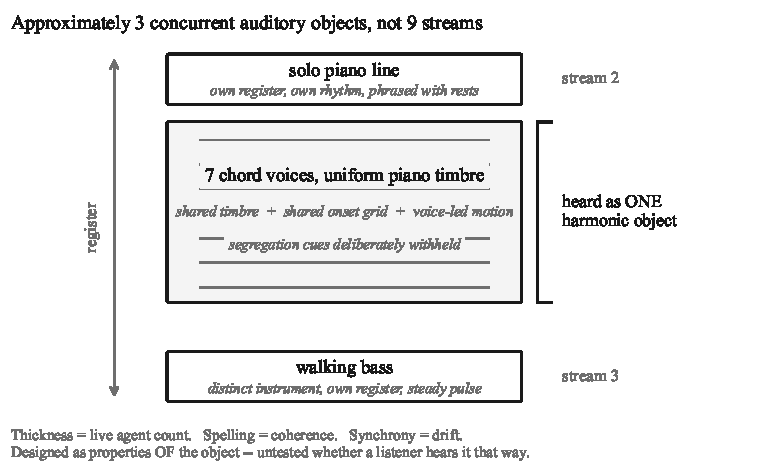
\includegraphics[width=\columnwidth]{figures/fig1_perceptual.pdf}
\caption{A design schematic, not a measurement. Seven chord voices share a timbre, an onset
grid, and voice-led motion, so the cues that would segregate them are deliberately withheld and
they are designed to fuse into one object. The solo line and bass are designed to stay
segregable, each violating those cues. Intended load is approximately three concurrent objects
rather than nine streams, with the oversight signals designed as properties of the fused object,
its thickness, spelling, and synchrony; whether a listener actually experiences it this way is
untested (Section~5).}
\label{fig:perceptual}
\end{figure}

\begin{figure}[t]
\centering
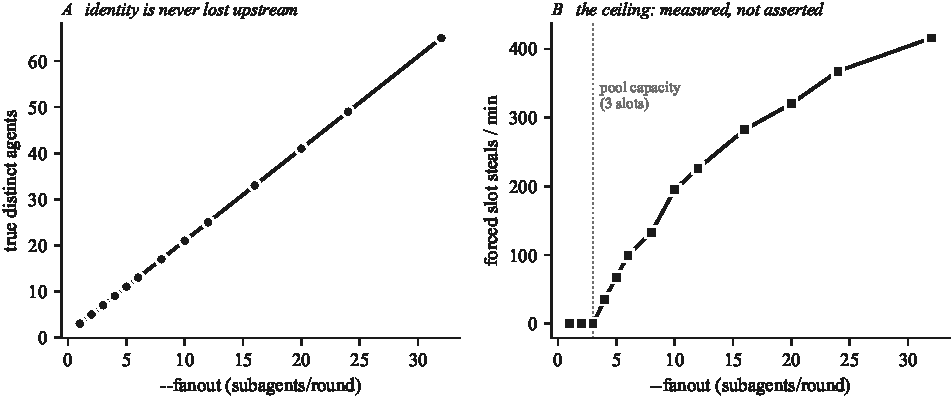
\includegraphics[width=\columnwidth]{figures/fig2_saturation.pdf}
\caption{The saturation ceiling. Panel A: true distinct agent count vs.\ \texttt{--fanout}, linear
with no cap. Panel B: forced pool-overflow events per minute vs.\ \texttt{--fanout}, with the
3-slot pool capacity marked; overflow is zero at or below capacity and rises monotonically above
it, from 0/min at fanout~3 to 415.9/min at fanout~32. Both averaged over 5 seeds per fanout value
(\texttt{make\_figures.py}).}
\label{fig:saturation}
\end{figure}

\begin{figure}[t]
\centering
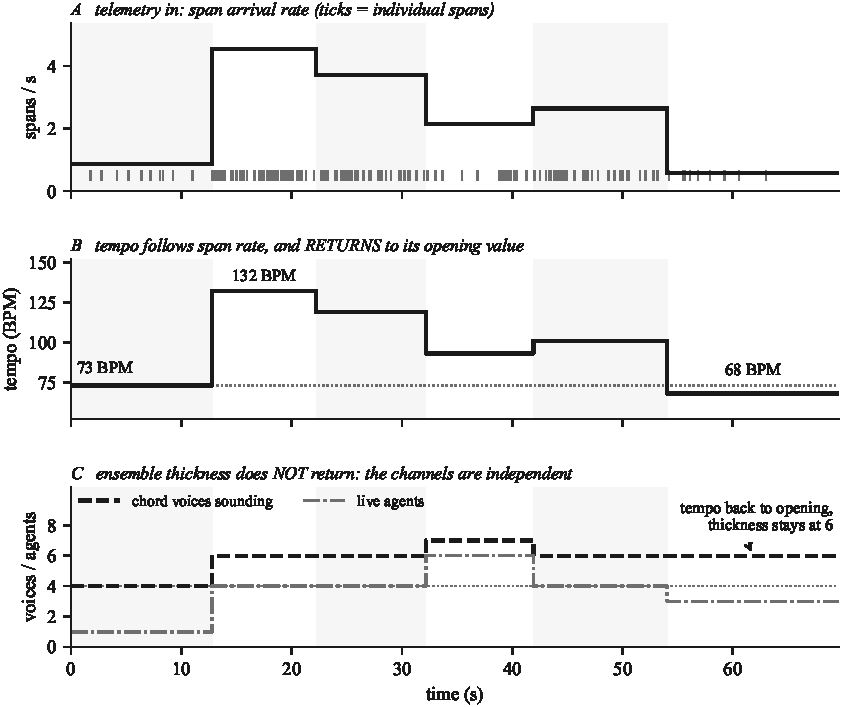
\includegraphics[width=\columnwidth]{figures/fig3_channels.pdf}
\caption{Telemetry in, two independent musical parameters out, for one swarm run
(\texttt{swarm.py}, seed~0, 153 spans over 69.6\,s; harmonic model
\texttt{corpus\_model\_jazz.json}; regenerate with \texttt{make\_figures.py --seed 0}). Panel A is
the input: individual span arrivals as ticks, with the per-movement arrival rate overlaid. Panel B
is tempo, which tracks span rate and returns to its opening value at convergence, 73~BPM down to
68~BPM. Panel C is ensemble thickness, which does not return: the chord stays at six voices
because agents remain live even as their span rate collapses. Movement boundaries are derived from
the telemetry, not authored. Every value plotted is measured from the engine's own exported note
events.}
\label{fig:channels}
\end{figure}
